
\begin{frame}{‌درخت پوشای کمینه}
\begin{itemize}\itemr
\item[-]
در طراحی مدارهای الکتریکی، معمولاً طراحان نیاز دارند که قسمت‌هایی از مدار را که در یک سطح ولتاژ قرار دارند، به یکدیگر متصل کنند. برای متصل کردن
\m{n}
نقطه به یکدیگر، به
\m{n-1}
سیم نیاز داریم که به شکل‌های متفاوت می‌توانند هر یک  دو نقطه را به یکدیگر متصل کنند. در چنین مسئله‌ای هدف یافتن روشی برای اتصال است که در آن از کمترین مقدار سیم لازم استفاده می‌کنیم. برای مدلسازی این مسئله به صورت زیر عمل می‌کنیم.
\item[-]
گراف
\m{G = (V,E)}
را با وزن‌های
\m{w : E \to \RR}
در نظر بگیرید. وزن یال
\m{(u,v) \in E}
برابر است با
\m{w(u,v)} .
\end{itemize}
\end{frame}


\begin{frame}{‌درخت پوشای کمینه}
\begin{itemize}\itemr
\item[-]
نقطه‌ها در یک مدار الکتریکی معادل رئوس گراف و سیم‌ها معادل یال‌های گراف هستند. مقدار سیمی که برای اتصال یک نقطه به نقطه دیگر نیاز است را با وزن یال مدلسازی می‌کنیم.
\item[-]
هدف پیدا کردن زیر مجموعهٔ
\m{ T \subseteq E}
است که همهٔ رئوس گراف را به یکدیگر متصل می‌کند و وزن کل آن برابر با
\m{w(T) = \sum_{(u,v) \in T} w(u,v)}
کمینه است.
\item[-]
زیرمجموعهٔ
\m{ T }
همهٔ رأس‌های گراف را به یکدیگر متصل می‌کند و دارای هیچ دوری نیست، پس یک درخت را تشکیل می‌دهد. به چنین درختی، درخت پوشا
\fn{1}{spanning tree}
گفته می‌شود. مسئله درخت پوشای کمینه
\fn{2}{minimum spanning tree problem}
به دنبال درخت پوشایی می‌گردد که وزن آن از همهٔ درخت‌های پوشای دیگر کمتر باشد.
\end{itemize}
\end{frame}


\begin{frame}{‌درخت پوشای کمینه}
\begin{itemize}\itemr
\item[-]
ورودی مسئله درخت پوشای کمینه گراف همبند بدون جهت
\m{G = (V,E)}
است که تابع وزن یال‌های آن
\m{w : E \rightarrow \RR}
است. هدف یافتن یک درخت پوشای کمینه برای
\m{G}
است.
\item[-]
دو الگوریتم حریصانه برای یافتن درخت پوشای کمینه معرفی خواهیم کرد که روش آنها مشابه است ولی پیاده‌سازی آنها متفاوت است.
\item[-]
این استراتژی را به عنوان یک الگوریتم کلی برای یافتن درخت پوشای کمینه معرفی می‌کنیم.
\end{itemize}
\end{frame}


\begin{frame}{‌درخت پوشای کمینه}
\begin{itemize}\itemr
\item[-]
الگوریتم کلی برای یافتن درخت پوشای کمینه به صورت زیر است.
\begin{algorithm}[H]\alglr
  \caption{Generic-MST} 
  \begin{algorithmic}[1]
   \Func{Generic-MST}{G,w}
   \State A =$\emptyset$
   \While{A does not form a spanning tree}
   			\State find an edge (u,v) that is safe for A
   			\State A = A $\cup$ {(u,v)}
   	\EndWhile
   	\State \Return A               
  \end{algorithmic}
  \label{alg:merge}
\end{algorithm}
\end{itemize}
\end{frame}


\begin{frame}{‌درخت پوشای کمینه}
\begin{itemize}\itemr
\item[-]
قبل از هر تکرار در حلقه،
\m{A}
یک زیر مجموعه از یک درخت پوشای کمینه است.
\item[-]
در هر گام از الگوریتم، یال
\m{(u,v)}
به
\m{A}
اضافه می‌شود بدون اینکه ویژگی
\m{A}
تغییر کند. به عبارت دیگر
\m{A \cup {(u,v)}}
نیز زیرمجموعه‌ای از درخت پوشای کمینه است.
\item[-]
یالی که به
\m{A}
اضافه می‌شود را یک یال مطمئن
\fn{1}{safe edge}
می‌نامیم زیرا ویژگی درخت را حفظ می‌کند.
\item[-]
پس در گام اول قبل از شروع حلقه ویژگی درخت (که زیرمجموعهٔ درخت پوشای کمینه است) برقرار است. در هرگام در حلقه تکرار ویژگی درخت حفظ می‌شود، پس در پایان یک درخت پوشای کمینه خواهیم داشت.
\end{itemize}
\end{frame}


\begin{frame}{‌درخت پوشای کمینه}
\begin{itemize}\itemr
\item[-]
حال روشی برای یافتن یال مطمئن ارائه می‌‌دهیم.
\item[-]
قبل از بررسی ویژگی یال مطمئن چند تعریف ارائه می‌کنیم.
\item[-]
یک برش
\fn{1}{cut}
\m{(S,V-S)}
از یک گراف بدون جهت
\m{G = (V,E)}
یک تقسیم‌بندی از رئوس
\m{V}
است که در آن مجموعهٔ رئوس به دو قسمت تقسیم می‌شوند.
\item[-]
می‌گوییم یال
\m{(u,v) \in E}
از برش
\m{(S,V-S)}
عبور می‌کند
\fn{1}{crosses}
اگر یک رأس یال در مجموعهٔ
\m{S}
و رأس دیگر یال در مجموعهٔ
\m{V-S}
قرار بگیرد.
\item[-]
یالی را که از یک برش عبور می‌کند یال سبک
\fn{3}{light edge}
می‌نامیم اگر وزن آن در بین همهٔ یال‌هایی که از برش عبور می‌کنند کمینه باشد. در یک برش ممکن است چند یال سبک هم‌وزن وجود داشته باشند.
\end{itemize}
\end{frame}


\begin{frame}{‌درخت پوشای کمینه}
\begin{itemize}\itemr
\item[-]
شکل زیر یک برش را نشان می‌دهد.
یال سبک در این برش یال 
\m{(c, d)}
با وزن ۷ است.
\begin{figure}
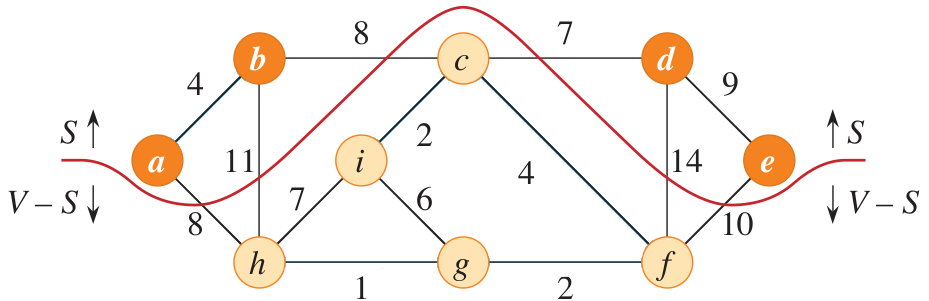
\includegraphics[width=0.9\textwidth]{figs/chap07/588-cut}
\end{figure}
\end{itemize}
\end{frame}


\begin{frame}{‌درخت پوشای کمینه}
\begin{itemize}\itemr
\item[-]
قضیه : فرض کنید
\m{G = (V,E)}
یک گراف همبند بدون جهت با یال‌های وزن‌دار باشد و وزن‌ها با تابع
\m{w}
تعریف شده باشند. فرض کنید
\m{A}
یک زیرمجموعه از
\m{E}
باشد که در یک درخت پوشای کمینه برای
\m{G}
قرار گرفته باشد و فرض کنید
\m{(S,V-S)}
یک برش از
\m{G}
باشد که هیچ یالی در
\m{A}
از آن
عبور نمی‌کند. فرض کنید
\m{(u,v)}
یک یال سبک باشد که از برش
\m{(S,V-S)}
عبور می‌کند. آنگاه یال
\m{(u,v)}
یک یال مطمئن برای
\m{A}
است.
\item[-]
اثبات:
از برهان خلف استفاده می‌کنیم.
فرض کنیم 
\m{(u,v)}
یک یال مطمئن برای 
\m{A}
نیست.
از آنجایی که 
درخت پوشای کمینه همبند است و در آن دور وجود ندارد، 
\m{u}
و
\m{v}
باید از طریق یک مسیر یکتا به یکدیگر متصل شده باشند.
حال یالی که 
\m{S}
و
\m{V-S}
را به یکدیگر متصل می‌کند از درخت پوشای کمینه حذف می‌کنیم و 
\m{(u,v)}
را جایگزین آن می‌کنیم. درخت پوشای به دست آمده هزینه‌اش از درخت قبلی بیشتر نیست و بنابراین کمینه است. پس یال
\m{(u,v)}
یک یال مطمئن است.
\end{itemize}
\end{frame}


\iffalse
\begin{frame}{‌درخت پوشای کمینه}
\begin{itemize}\itemr
\item[-]
اثبات : فرض کنید
\m{T}
یک درخت پوشای کمینه باشد که
\m{A}
را شامل می‌شود. درخت پوشای کمینه
\m{T'}
را به گونه‌ای می‌سازیم که شامل
\m{A \cup {(u,v)}}
شود و نشان می‌دهیم که
\m{(u,v)}
یک یال مطمئن برای
\m{A}
است.
\item[-]
از آنجایی که 
درخت پوشای کمینه همبند است و در آن دور وجود ندارد، 
\m{u}
و
\m{v}
باید از طریق یک مسیر یکتا به یکدیگر متصل شده باشند.
 مسیر ساده
\m{p}
از رأس
\m{u}
به
\m{v}
در درخت
\m{T}
را در نظر بگیرید.
\item[-]
شکل زیر این حالت را نشان می‌دهد.
\begin{figure}
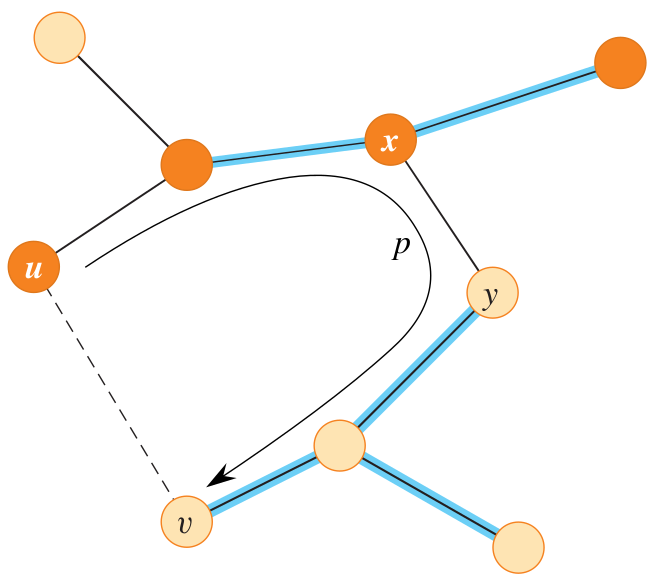
\includegraphics[width=0.3\textwidth]{figs/chap07/589-proof}
\end{figure}
\end{itemize}
\end{frame}


\begin{frame}{‌درخت پوشای کمینه}
\begin{itemize}\itemr
\item[-]
از آنجایی که
\m{u}
و
\m{v}
در دو طرف برش
\m{(S,V-S)}
قرار دارند، حداقل یک یال در
\m{T}
وجود دارد که بر روی مسیر سادهٔ
\m{p}
است و همچنین از برش عبور می‌کند. فرض کنید
\m{(x,y)}
چنین یالی باشد.
\item[-]
یال
\m{(x,y)}
در
\m{A}
نیست، زیرا می‌دانیم برش از یال‌های
\m{A}
عبور نمی‌کند.
\item[-]
از آنجایی که
\m{(x,y)}
یک مسیر ساده یکتا از
\m{u}
به
\m{v}
در
\m{T}
است، حذف کردن
\m{(x,y)}
درخت
\m{T}
را به دو جزء تقسیم می‌کند. اضافه کردن
\m{(u,v)}
آن دو جزء را دوباره به یکدیگر متصل می‌کند و درخت پوشای جدید
\m{T' = (T - \{(x,y)\}) \cup \{(u,v)\}}
را می‌سازد.
\end{itemize}
\end{frame}


\begin{frame}{‌درخت پوشای کمینه}
\begin{itemize}\itemr
\item[-]
حال نشان می‌دهیم
\m{T'}
یک درخت پوشای کمینه است. از آنجایی که
\m{(u,v)}
یک یال سبک است که از
\m{(S,V-S)}
عبور می‌کند و
\m{(x,y)}
نیز از این برش عبور می‌کند
\m{w(u,v) \leqslant w(x,y)}
. بنابراین :
\begin{align*}
\m{w(T') = w(T) - w(x,y) + w(u,v) \leqslant w(T)}
\end{align*}
\item[-]
اما
\m{T}
یک درخت پوشای کمینه است، بنابراین
\m{w(T) \leqslant w(T')}
و بنابراین
\m{T'}
باید یک درخت پوشای کمینه باشد.
\item[-]
حال باید نشان دهیم
\m{(u,v)}
یک یال سبک برای
\m{A}
است. داریم
\m{A \subseteq T'}
بنابراین
\m{A \subseteq T}
و
\m{(x,y) \notin A}
بنابراین
\m{A \cup{(u,v)} \subseteq T'}
بنابراین از آنجایی که
\m{T'}
یک درخت پوشای کمینه است،
\m{(u,v)}
برای
\m{A}
مطمئن است.
\end{itemize}
\end{frame}
\fi